\definecolor{CeShiftIdentityPoints}{HTML}{2878B5}
\definecolor{CeShiftIdentityLine}{HTML}{E37A26}

% #1 title, #2 data, #3 minimum, #4 maximum, #5 annotation.
\newcommand{\CeShiftIdentityPlot}[5]{%
  \begin{minipage}[t]{0.47\textwidth}
    \centering
    {\small\bfseries #1\par}
    \vspace{0.1em}
    \begin{tikzpicture}
      \begin{axis}[
        width=5.55cm,
        height=5.55cm,
        scale only axis,
        xmin=#3,
        xmax=#4,
        ymin=#3,
        ymax=#4,
        xlabel={$\overline{\mathrm{CE}}_{\mathrm{atomic}}(\mathbf{x})$},
        ylabel={$\overline{\mathrm{CE}}_{\mathrm{joint}}(\mathbf{x})$},
        scaled x ticks=false,
        scaled y ticks=false,
        tick label style={font=\scriptsize},
        label style={font=\scriptsize},
        grid=major,
        grid style={gray!18},
        axis line style={gray!60},
        clip=true,
      ]
        \addplot[
          scatter,
          only marks,
          mark=*,
          draw=CeShiftIdentityPoints,
          fill=CeShiftIdentityPoints,
          fill opacity=0.62,
          scatter/use mapped color={
            draw=CeShiftIdentityPoints,
            fill=CeShiftIdentityPoints
          },
          visualization depends on={\thisrow{marker_size}\as\perpointmarksize},
          scatter/@pre marker code/.append style={/tikz/mark size=\perpointmarksize pt},
        ] table[
          col sep=comma,
          x=atomic_ce,
          y=interaction_ce,
          meta=concept_count
        ] {#2};
        \addplot[
          CeShiftIdentityLine,
          very thick,
          dashed,
          domain=#3:#4,
          samples=2
        ] {x};
      \end{axis}
    \end{tikzpicture}
    \vspace{-0.2em}
    {\scriptsize #5\par}
  \end{minipage}%
}

\newcommand{\CeShiftConceptCountLegend}{%
  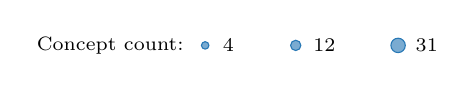
\begin{tikzpicture}[baseline=-0.6ex]
    \node[anchor=east,font=\scriptsize] at (-0.15,0) {Concept count:};
    \foreach \x/\size/\label in {0/1.35/4,1.15/1.86/12,2.45/2.60/31}{
      \draw[CeShiftIdentityPoints,fill=CeShiftIdentityPoints,fill opacity=0.62]
        (\x,0) circle[radius=\size pt];
      \node[anchor=west,font=\scriptsize] at (\x+0.10,0) {$\label$};
    }
  \end{tikzpicture}%
}

\begin{figure}[p]
  \centering
  \CeShiftIdentityPlot{BBQ --- GPT-OSS 120B}%
    {data/appendix/ce_shift_identity/bbq_gptoss.csv}{0}{0.6}%
    {$n=30$ questions; $k=4$--$6$ concepts}
  \hfill
  \CeShiftIdentityPlot{BBQ --- Mistral Medium 3.5}%
    {data/appendix/ce_shift_identity/bbq_mistral.csv}{0}{0.6}%
    {$n=30$ questions; $k=4$--$6$ concepts}

  \par\vspace{1.1em}
  \CeShiftIdentityPlot{MedQA --- GPT-OSS 120B}%
    {data/appendix/ce_shift_identity/medqa_gptoss.csv}{0}{0.06}%
    {$n=29$ questions; $k=8$--$31$ concepts}
  \hfill
  \CeShiftIdentityPlot{MedQA --- Mistral Medium 3.5}%
    {data/appendix/ce_shift_identity/medqa_mistral.csv}{0}{0.06}%
    {$n=24$ questions; $k=6$--$16$ concepts}

  \par\vspace{0.7em}
  \CeShiftConceptCountLegend
  \caption[Question-level CE agreement under atomic and joint attribution]{Question-level mean causal effects under atomic and interaction-aware attribution for BBQ and MedQA. The dashed line denotes equality. Marker area increases with the number of concepts contributing to the question-level mean.}
  \label{fig:appendix-ce-shift-identity-natural-language}
\end{figure}

\begin{figure}[p]
  \centering
  \CeShiftIdentityPlot{New German Credit --- GPT-OSS 120B}%
    {data/appendix/ce_shift_identity/new_german_credit_gptoss.csv}{0}{1.5}%
    {$n=30$ questions; $k=12$ concepts}
  \hfill
  \CeShiftIdentityPlot{New German Credit --- Mistral Medium 3.5}%
    {data/appendix/ce_shift_identity/new_german_credit_mistral.csv}{0}{1.5}%
    {$n=30$ questions; $k=12$ concepts}

  \caption[Question-level CE agreement for New German Credit]{Question-level mean causal effects under atomic and interaction-aware attribution for New German Credit. Every question contains the same 12 concepts, so marker size is constant.}
  \label{fig:appendix-ce-shift-identity-credit}
\end{figure}
